\chapter{Pregled područja}
\label{ch:pregled-podrucja}
Ovo poglavlje ukratko opisuje povijest raspoznavanja teksta, podjelu područja raspoznavanja teksta te često korištene
pristupe problemu. Također su opisani pristupi korišteni u nekoliko odabranih znanstvenih članaka. Na prvi pogled se
raspoznavanje teksta može činiti kao jednostavan problem, međutim čak i ljudsko oko ima pogrešku raspoznavanja oko 4\%
pri raspoznavanju znakova bez konteksta \citep{mantas1986}. Raspoznavanje teksta ima broje primjene, kao što su čitači
teksta koje pomažu slijepim i slabovidnim osobama, telekomunikacijski uređaji za gluhonijeme osobe, očitavanje adresa u
poštanskim uredima, očitavanje dokumenata, automatsko raspoznavanje brojeva na automobilskim tablicama, te mnoge druge
\citep{govindan1989}.


\section{Povijesni pregled}
\label{sec:povijesni-pregled}
Područje raspoznavanja teksta podskup je područja raspoznavanja uzoraka. Podrijetlo područja raspoznavanja teksta može
se pronaći još u 19. stoljeću \citep{mantas1986}, kada je američki izumitelj Charles R. Carey 1870. godine izumio stroj
za skeniranje retine. Ovo se smatra prvim izumom u području raspoznavanja teksta. Međutim, prva primjena raspoznavanja
teksta pojavila se kao pomagalo za slijepe i slabovidne osobe koju je 1900. primijenio ruski znanstvenik Tyurin
\citep{govindan1989}. Područje se neprestano razvijalo kroz sljedećih nekoliko desetljeća, te se pojavom digitalnih
računala sredinom 1940-ih godina razvija moderna inačica optičkog raspoznavanja teksta. Jedan od najranijih pokušaja
raspoznavanja teksta opisan je u radu R. L. Grimsdale i ostalih pod naslovom
\emph{``A system for automatic recognition of patterns''}, 1959. godine. Ranih 1960-ih godina, američki znanstvenik
Murray Eden predstavio je ideju da se svi latinični znakovi mogu formirati od maksimalno 18 poteza, koji se nadalje mogu
formirati od podskupa 4 segmenata. Ovaj koncept zaslužan je za uspostavu metode analize koristeći sintezu, međutim
njegova je veća važnost ta što je formalno dokazano da se rukom pisani znakovi mogu formirati iz konačnog skupa
značajki \citep{mantas1986}. Mogućnost dekompozicije znakova u manje cjeline sretna je okolnost za područje
raspoznavanja teksta jer svaka cjelina može doprinijeti neku značajnost u postupku raspoznavanja \citep{mori1999}.


\section{Podjela područja}
\label{sec:podjela-podrucja}
Područje raspoznavanja teksta može su podijeliti na tri dijela: magnetsko raspoznavanje teksta, mehaničko raspoznavanje
teksta te optičko raspoznavanje teksta. Magnetsko i mehaničko raspoznavanje teksta neće se dalje razmatrati u ovome
radu te će fokus biti na optičkom raspoznavanju teksta. Optičko raspoznavanje teksta u širem smislu spada pod granu
umjetne inteligencije \citep{mori1999} te se dalje može podijeliti na:
\begin{enumerate}
    \item \emph{Raspoznavanje znakova fiksne širine}. Ovaj dio područja bavi se raspoznavanjem pojedinih znakova
    tiskanog teksta.
    \item \emph{On-line raspoznavanje teksta} je raspoznavanje rukom pisanih znakova gdje slika svakog znaka dolazi uz
    vremensku informaciju svakog poteza rukom.
    \item \emph{Raspoznavanje rukom pisanih znakova} je raspoznavanje pojedinih rukom pisanih znakova koji nisu spojeni
    niti pisani u kurzivu.
    \item \emph{Raspoznavanje rukom pisanog teksta} je raspoznavanje pojedinih rukom pisanih znakova bez ikakvih
    ograničenja stila pisanja. Znakovi mogu biti spojeni i pisani kurzivnim stilom.
\end{enumerate}
Raspoznavanje znakova fiksne širine dalje se može podijeliti na raspoznavanje znakova specifičnog fonta, raspoznavanje
znakova više različitih fontova i raspoznavanje znakova bilo svih fontova \citep{govindan1989}.
Slika \ref{fig:podjela-podrucja-raspoznavanja-teksta} prikazuje podjelu područja raspoznavanja teksta na tri glavna
dijela te detaljnu podjelu područja optičkog raspoznavanja teksta. Slika je preuzeta i prilagođena
iz \citep{mantas1986}.

\begin{figure}[htb]
    \centering
    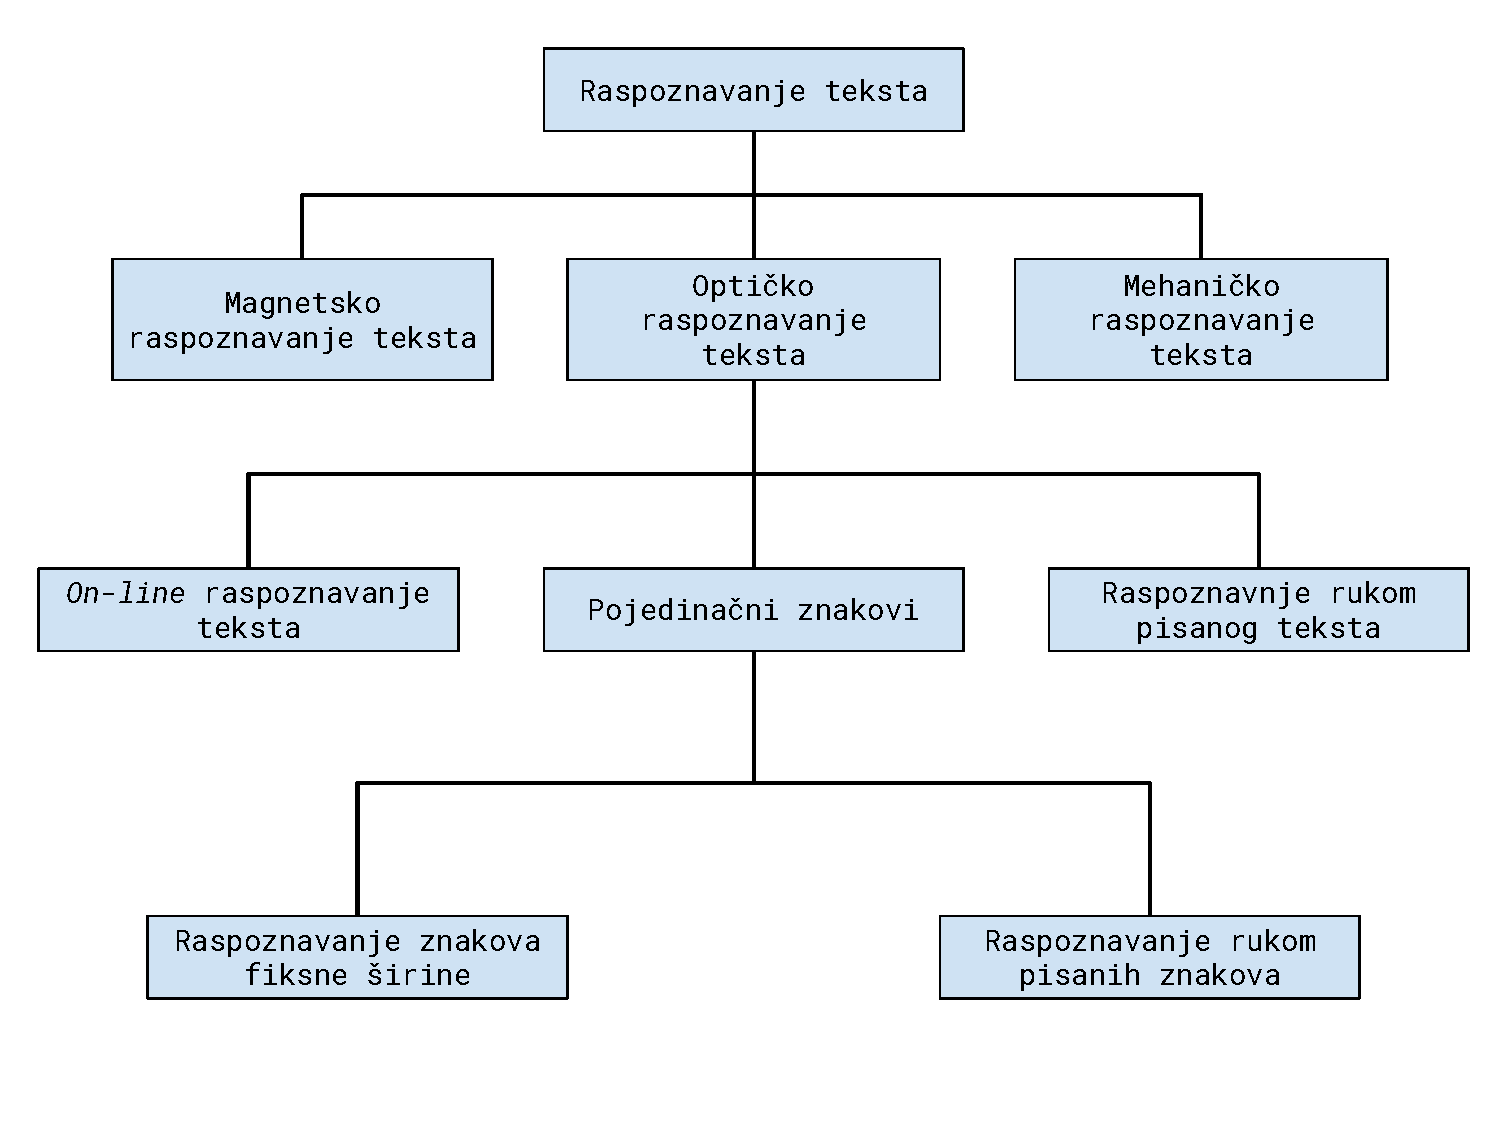
\includegraphics[width=12cm]{images/character-recognition-categories.pdf}
    \caption{Podjela područja raspoznavanja teksta}
    \label{fig:podjela-podrucja-raspoznavanja-teksta}
\end{figure}

S obzirom na korištene značajke, tehnike raspoznavanja teksta možemo razvrstati u dvije kategorije \citep{govindan1989}:
\begin{enumerate}
    \item \emph{Tehnika korelacije i podudaranja predložaka}
    \item \emph{Tehnika analize i podudaranja značajki}
\end{enumerate}
Kod tehnike korelacije i podudaranja predložaka ulazni znakovi se uspoređuju sa skupom predložaka znakova te se
klasifikacija obavlja na temelju sličnosti. Metoda usporedbe znakova može biti veoma jednostavna, kao što je usporedba
svakog pojedinog odgovarajućeg piksela, ili komplicirana, kao na primjer usporedba koristeći stablo odluke koje određuje
koji pikseli će se uspoređivati. Glavni nedostatak ove tehnike je neotpornost na ulazne smetnje i varijaciju u stilu
pisanja. Tehnika analize i podudaranja značajki češće je korištena tehnika raspoznavanja teksta. Ova tehnika
podrazumijeva odabir odgovarajućih značajki koje se uspoređuju sa značajkama idealnih znakova te se znak čije se
značajke najviše podudaraju s ulaznim primjerom dodjeljuje kao prepoznati znak \citep{govindan1989}.


\section{Pristupi problemu raspoznavanja teksta}
\label{sec:pristupi-problemu-raspoznavanja-teksta}
U području raspoznavanja uzoraka postoje dva glavna pristupa: prvi pristup je statistički ili teoretski pristup, a drugi
pristup je sintaktički ili strukturni pristup \citep{govindan1989}. Svaki od navedenih pristupa ima svoje prednosti i
mane. Na primjer, kod kompleksnih uzoraka statistički pristup ne može dovoljno precizno opisati informacije o međusobnim
strukturnim vezama između komponenti te time gubi na preciznosti pri raspoznavanju. S druge strane, sintaktički pristup
ne može u potpunosti opisati ulazne uzorke na temelju strukturnih modela znakova. Uzorci su prirodne pojave koje se ne
mogu uvijek u potpunosti opisati matematičkim i formalnim jezikom. Zbog toga, za raspoznavanje teksta potrebne su
tehnike za opisivanje velikog broja sličnih struktura iste kategorije dok istovremeno dozvoljavamo različite opise
među kategorijski različitim uzorcima \citep{govindan1989}. Pristup problemu raspoznavanja znakova također možemo
podijeliti ovisno o korištenoj metodologiji. Metodologije za raspoznavanje teksta mogu se svrstati u sljedećih 6
kategorija \citep{mantas1986}:
\begin{enumerate}
    \item \emph{Globalna usporedba točaka} - pikseli ulazne slike uspoređuju se sa svim pikselima baze znakova.
    \item \emph{Globalne transformacije} - kao značajke odabiru se vrijednosti dobivene koristeći neku od globalnih
    transformacija nad ulaznom slikom, kao na primjer \emph{Karhunen-Loèveova} ili \emph{Fourierova} transformacija.
    \item \emph{Odabir lokalnih značajki} - pod ovu kategoriju spadaju značajke dobivene analizom krajnjih točaka
    znakova, točaka presjecišta linija, vrijednosti kuteva među linijama te ostalim sličnim metodama. Često je potrebno
    stanjiti ulazne znakove prije određivanja vrijednosti značajki.
    \item \emph{Odabir značajki koristeći linije} - koriste se vertikalne, horizontalne te dijagonalne linije kako bi
    se odredile vrijednost značajki.
    \item \emph{Analiza krivulja} - značajke se određuju preko smjera krivulja i geometrijske analize.
    \item \emph{Strukturna analiza} - ulazni znakovi rastavljaju se na manje gradivne komponente koje se zatim
    reduciraju u graf koji opisuje topologiju znaka.
\end{enumerate}
Neovisno o odabranoj metodologiji, proces raspoznavanja teksta može se ugrubo podijeliti u tri dijela: pretprocesiranje,
odabir značajki te klasifikacija \citep{mori1999}. Pretprocesiranje je korak je čija se važnost često zanemari u odnosu
na preostala dva koraka, ali ono je podjednako važno. Kvalitetno pretprocesiranje može značajno smanjiti kompleksnost
ulazne slike te time olakšati proces odabira značajki, što će dalje pridonijeti boljoj klasifikaciji.


\section{Analiza postojećih radova}
\label{sec:analiza-postojecih-radova}
Ovaj rad bavi se raspoznavanjem rukom pisanih znamenaka, koje je podskupom problema raspoznavanja ručno pisanog teksta.
Raspoznavanje rukom pisanog teksta podrazumijeva da ne postoje ograničenja stila pisanja i odvojivosti znakova
\citep{mantas1986}. Ovaj odjeljak analizira nekoliko znanstvenih radova koji nude razne pristupe navedenom problemu.
% TODO up is done
% TODO
